\documentclass[10pt,a4paper]{article}
\usepackage[T1]{fontenc}
\usepackage{mathptmx}
\usepackage[a4paper,margin=1.7cm]{geometry}
\usepackage{graphicx}
\usepackage[font=small,labelfont=bf,labelsep=period,skip=3pt]{caption}
\usepackage{enumitem}
\setlist{itemsep=1pt,topsep=2pt,leftmargin=1.4em}
\usepackage{microtype}
\setlength{\parindent}{0pt}
\setlength{\parskip}{3pt}
\setlength{\textfloatsep}{8pt}
\setlength{\floatsep}{8pt}
\setlength{\intextsep}{6pt}
\newcommand{\x}{$\times$}
\makeatletter\setlength{\@fptop}{0pt}\setlength{\@fpsep}{10pt}\makeatother
\renewcommand{\topfraction}{0.95}\renewcommand{\bottomfraction}{0.9}
\renewcommand{\textfraction}{0.05}\renewcommand{\floatpagefraction}{0.6}

\begin{document}

{\Large\bfseries Pre-read, gradual pruning of wider Nequix models}\\[2pt]
{\large Latest results since the last meeting \hfill 24 November 2026}
\par\smallskip\hrule

\subsection*{Setup}
\begin{itemize}
  \item We widen the tensor products of Nequix-MP-1 by a factor $k$ (1.25, 1.5, 2, 2.5 or 3) and prune the model
        gradually during training with BM-$\mu$, in 6 steps (epochs 30 to 75), down to the size of Nequix-MP-1.
        We measure size as the number of tensor-product paths (3,236 for Nequix-MP-1), the quantity our pruning
        budget controls. Each model then recovers for 25 epochs.
  \item The baseline is Nequix-MP-1 trained directly, without pruning. All runs share the same recipe (MPtrj, BMuon,
        learning rate 0.01, weight decay $10^{-3}$, batch 256, 100 epochs, same seed). Errors are on the validation
        split (79,020 structures), with one seed per model.
\end{itemize}

\subsection*{Key results}
\begin{enumerate}
  \item Gradually pruning a 1.5\x\ wider Nequix down to the size of Nequix-MP-1 gives a better model than training
        Nequix-MP-1 directly, with a 1.4\,\% lower force error (95\,\% CI $-1.7$ to $-1.1$\,\%) and a 4.7\,\% lower
        energy error (95\,\% CI $-5.3$ to $-4.1$\,\%) (Fig.~3).
  \item Starting wider than 1.5\x\ does not help. 2\x\ and 2.5\x\ end within 0.6\,\% of Nequix-MP-1 on forces and
        3.3\,\% below it on energy, 3\x\ is still training, and 1.25\x\ is worse than Nequix-MP-1 (Figs.~1 and 2).
        We think the wider models need more recovery time, since each pruning step removes a larger share of them
        (7\,\% of the remaining size at 1.5\x, 17\,\% at 3\x) and their error jumps more after each step.
        We kept the same schedule for all widths because training is already heavy, so whether longer recovery is
        worth the extra cost is open for discussion.
  \item The price is a small loss in efficiency. The pruned 1.5\x\ model is about 8\,\% slower at inference (2.28 vs
        2.12 ms per structure) and has 5\,\% more parameters (Fig.~3c). Training also costs more, since the wider model
        is trained at full width.
  \item We also retrained the architecture found by pruning from scratch, but for now it is not going great. At epoch 26
        of 99 it is about 1\,\% behind Nequix-MP-1 on both forces and energy (Fig.~4).
\end{enumerate}

\begin{figure}[!htb]
\centering
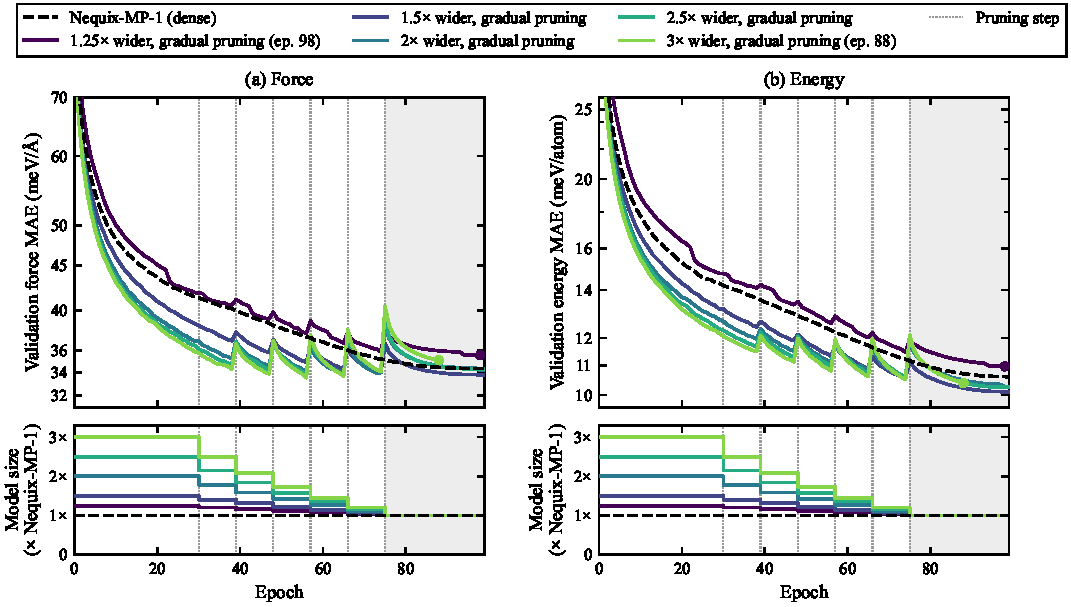
\includegraphics[width=0.66\textwidth]{fig1_gradual-pruning-of-wider-models_training-curves.pdf}
\caption{Validation error during training of the $k$\x\ wider models, gradually pruned to the size of Nequix-MP-1.
Dotted lines mark the pruning steps and the shaded area the epochs where all models have the size of Nequix-MP-1.
The bottom panels show the model size (number of tensor-product paths) relative to Nequix-MP-1. Log scale, dots mark runs still training.}
\end{figure}

\begin{figure}[!htb]
\centering
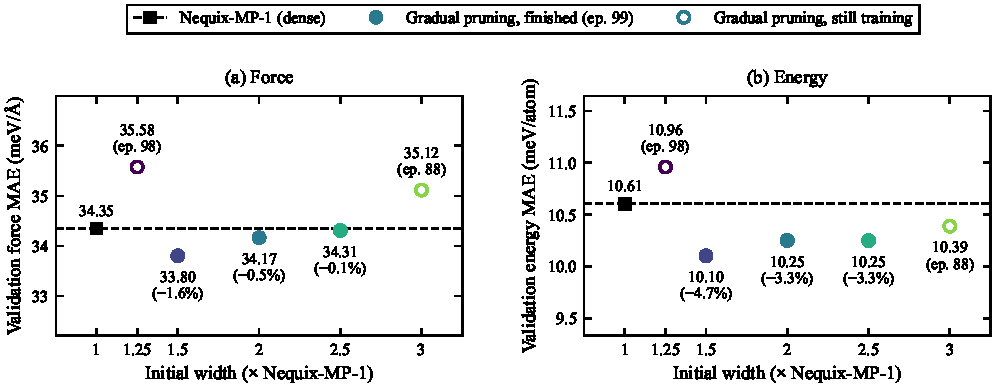
\includegraphics[width=0.64\textwidth]{fig2_final-error-vs-width.pdf}
\caption{Validation error at the last epoch against the initial width. Filled markers are finished runs (epoch 99)
with their difference to Nequix-MP-1, open markers are runs still training at their latest epoch.}
\end{figure}

\begin{figure}[!htb]
\centering
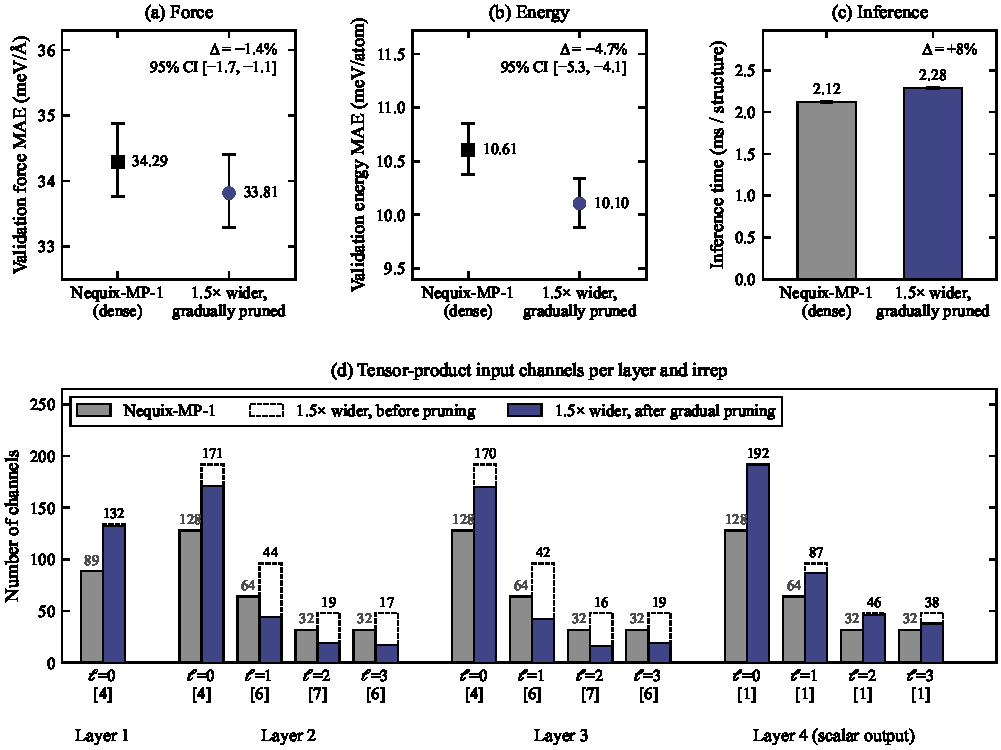
\includegraphics[width=0.82\textwidth]{fig3_x1.5-pruned-vs-dense_equal-cost.pdf}
\caption{The 1.5\x\ wider model after gradual pruning against Nequix-MP-1, at epoch 99. (a, b) Whole validation split,
error bars are 95\,\% bootstrap intervals and $\Delta$ uses a paired bootstrap. (c) Energy and forces, batches of 32,
one RTX 2000 Ada GPU, pruned channels removed. (d) Channels entering each tensor product, with the number of
tensor-product paths fed by each channel in brackets. The last layer outputs scalars only, so its channels feed one
path each.}
\end{figure}

\begin{figure}[!htb]
\centering
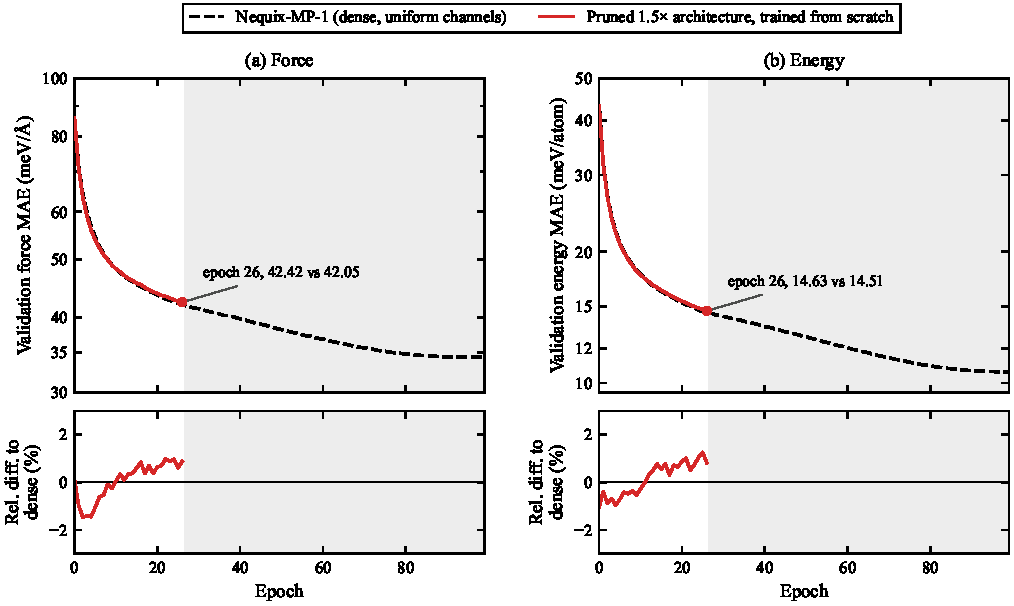
\includegraphics[width=0.66\textwidth]{fig4_pruned-architecture-from-scratch.pdf}
\caption{The architecture found by pruning the 1.5\x\ model (Fig.~3d), trained from scratch without pruning, against
Nequix-MP-1, with the same recipe and seed. The bottom panels show the relative difference at the same epoch, the
shaded area the epochs not reached yet.}
\end{figure}

\end{document}
